\documentclass[5p,times]{elsarticle}

\usepackage{graphicx}
\usepackage{url}
\usepackage{upgreek}
\usepackage{epstopdf}
\usepackage{bm}
\usepackage{amsmath,amssymb}
\usepackage{array}
\usepackage{float}
\newcolumntype{L}[1]{>{\raggedright\arraybackslash}p{#1}}
\renewcommand{\figurename}{Fig.}
\biboptions{sort&compress}
\journal{International Journal of Non-Linear Mechanics}
\emergencystretch=3em
\clubpenalty=0
\widowpenalty=0
\displaywidowpenalty=0

\newcommand{\figplaceholder}[3]{%
  \IfFileExists{#1}{%
    \includegraphics[width=#2]{#1}%
  }{%
    \fbox{%
      \rule{0pt}{#3}\rule{#2}{0pt}%
    }%
  }%
}

\begin{document}

\begin{frontmatter}

\title{Model Predictive Control for Bipedal Robots Based on a Variable-Inertia Centroidal Model}

\author[label1]{Junwei Mei}
\author[label1]{Xinrui Li}
\author[label1]{Jiawei Xie}
\author[label1,label2,label3]{Xiaoxu Zhang\corref{cor1}}
\ead{zhangxiaoxu@fudan.edu.cn}
\author[label1,label2,label3]{Jian Xu}
\cortext[cor1]{Corresponding author.}
\address[label1]{College of Intelligent Robotics and Advanced Manufacturing, Fudan University, Shanghai 200433, China}
\address[label2]{MOE Frontiers Center for Brain Science, Fudan University, Shanghai 200433, China}
\address[label3]{Yiwu Research Institute, Fudan University, Yiwu 322000, China}

\begin{abstract}
The single rigid body model is widely used in model predictive control for bipedal robots because of its compact structure and real-time computational efficiency. However, its constant-inertia assumption cannot fully capture the influence of configuration-dependent swing-leg inertia on whole-body angular dynamics. This paper proposes a model predictive control method based on a variable-inertia centroidal model for bipedal locomotion. The proposed model updates the whole-body centroidal inertia online and incorporates the effect of inertia variation on angular-velocity evolution within a low-dimensional centroidal prediction model, while preserving the same contact-wrench input structure as the single rigid body model. The resulting control framework combines contact-constrained model predictive control, Raibert-type foot placement, and whole-body control to coordinate stance contact, torso regulation, and swing-leg motion. Simulation results show that, for low two-leg mass fractions and velocity-tracking tasks, the single rigid body model remains highly effective when closed-loop feedback and whole-body control are present. The benefit of the variable-inertia centroidal model is mainly observed in boundary conditions with large leg inertia, pronounced turning-induced angular-momentum variation, or external disturbance recovery, where it improves angular-dynamics prediction consistency and enlarges the stability margin in selected scenarios.
\end{abstract}

\begin{keyword}
Biped robot \sep Variable-inertia centroidal model \sep Model predictive control \sep Whole-body control \sep Dynamic locomotion
\end{keyword}

\end{frontmatter}

\section{Introduction}
Legged robots, especially bipedal and humanoid robots, are regarded as important platforms for mobile operation in complex environments because their geometric scale and contact mode are naturally compatible with human-centered surroundings. Compared with wheeled or tracked platforms, legged systems have greater potential for confined-space traversal, discrete-terrain locomotion, inspection in complex scenes, and service or interaction tasks in human environments \cite{ref22,ref23,ref20,ref74,ref78}. Therefore, stable, efficient, and dynamically capable locomotion control for bipedal robots is not only of clear engineering importance, but also constitutes a fundamental research problem at the intersection of robot dynamics, control, and optimization.

Existing control strategies for bipedal robots can be broadly divided into model-based methods and data-driven methods that do not rely on an exact analytical model. The former originated from the zero-moment point (ZMP) and linear inverted pendulum model (LIPM), and has gradually evolved into systematic frameworks based on hybrid zero dynamics, centroidal dynamics, momentum control, and whole-body control \cite{ref12,ref17,ref18,ref14,ref16,ref25,ref36,ref55,ref63}. The latter is represented by deep reinforcement learning, imitation learning, and hybrid learning-control strategies, which generate complex gait behaviors through large-scale interaction or human priors and have shown substantial potential in terrain adaptation, natural gait transfer, and simulation-to-real deployment \cite{ref56,ref58,ref59,ref62}. Although data-driven methods have demonstrated frontier capabilities in behavioral emergence and policy generalization, model-based methods remain indispensable for bipedal robots, which are highly constrained, multi-contact, and safety-critical systems. In particular, model predictive control (MPC) can explicitly handle state evolution and contact constraints over a finite prediction horizon, whereas whole-body control (WBC) can consistently map high-level centroidal decisions to full-body multi-task execution. For this reason, this paper adopts a hierarchical MPC--WBC framework as the main control architecture.

Within the model-based paradigm, the development of MPC has been accompanied by an evolution of prediction models from highly simplified representations toward higher-fidelity formulations. Early studies mainly employed LIPM or ZMP preview models to generate real-time feasible gait patterns with a low-dimensional state representation \cite{ref17,ref18,ref19}. Later, centroidal dynamics and the single rigid body model (SRBM) were introduced to include contact forces, contact moments, and angular-momentum variation in the prediction process, thereby improving the representation of multi-contact dynamics \cite{ref25,ref44,ref49,ref50}. More recently, nonlinear MPC, whole-body MPC, adaptive-complexity MPC, and multi-fidelity prediction methods have further extended the applicability of MPC to highly dynamic motion, complex terrain, and whole-body coordination \cite{ref31,ref51,ref52,ref53,ref54,ref35,ref42,ref77}. Nevertheless, low-dimensional MPC schemes commonly used for online control still rely on constant-inertia or weak-coupling assumptions. In particular, SRBM-based controllers usually neglect the time-varying contribution of swinging limbs to the centroidal inertia of the whole robot \cite{ref29,ref39,ref40}. This limitation becomes more pronounced in fast walking, large-step locomotion, high-speed leg swing, and disturbance-recovery scenarios. On the one hand, mass redistribution caused by the swing leg changes the inertia tensor about the system center of mass. On the other hand, inertia variation directly affects angular-velocity evolution, producing angular-dynamics modeling errors that are not represented by conventional SRBM. As a result, the optimal contact forces computed by MPC may deviate systematically from the forces required by the real multi-body system, degrading centroidal tracking, weakening attitude stability, and even causing contact-allocation errors and gait failure. Directly using full-body dynamics can improve physical fidelity, but it also substantially increases the optimization dimension and computational burden, which is unfavorable for high-frequency online control \cite{ref77}.

To address this issue, this paper proposes a bipedal MPC method based on a variable-inertia centroidal model (VICM). At the modeling level, the method computes the configuration-dependent centroidal inertia tensor online and incorporates the effect of inertia variation on angular-velocity evolution into a low-dimensional prediction model expressed in a world-aligned inertial frame. At the predictive-control level, it formulates a linearized MPC problem with state-tracking and control-regularization costs, while systematically including friction-cone, unilateral-contact, support-area, and gait-phase constraints. At the execution level, WBC is used to enforce contact consistency, torso regulation, foot-force distribution, and swing-leg tracking. The proposed method preserves the online efficiency of low-dimensional MPC while improving the representation of real centroidal dynamics under fast leg swing and dynamic gait conditions, thereby providing a more consistent prediction model for scenarios with significant angular-momentum variation.

The remainder of this paper is organized as follows. Section 2 presents the construction of the bipedal robot dynamics model. Section 3 introduces the MPC controller, swing-leg trajectory generation, and WBC design based on the proposed model. Section 4 presents simulation results and comparative analysis. Section 5 concludes the paper and discusses future work.

\section{Bipedal Robot Dynamics}
To balance real-time predictability and dynamic fidelity, this paper follows the basic idea of centroidal dynamics modeling for bipedal robots. A single rigid body model is first introduced as a low-dimensional baseline model for online optimization. Then, while keeping the control-input dimension unchanged, configuration-dependent inertia is incorporated into the centroidal angular-momentum equation to construct the variable-inertia centroidal model. The sign conventions used in the dynamics formulation are shown in Fig.~\ref{fig:sign_conventions}. Unless otherwise stated, the CoM and contact positions, CoM linear velocity, base angular velocity, contact wrenches, centroidal angular momentum, and centroidal inertia tensor used in the centroidal dynamics are expressed in a world-aligned inertial frame. The attitude state $\bm\Theta=[\phi,\theta,\psi]^\top$ is represented by roll-pitch-yaw coordinates, whose rate is related to the angular velocity through the small-roll/pitch approximation introduced below. Let the total robot mass be $m$, the center-of-mass (CoM) position be $\bm c\in\mathbb{R}^3$, the CoM linear velocity be $\bm v=\dot{\bm c}$, the base angular velocity be $\bm\omega\in\mathbb{R}^3$, the position of the $k$th contact point be $\bm p_k$, and the corresponding contact force and contact moment be $\bm f_k$ and $\bm\tau_k$, respectively.
\begin{figure}[t]
\centering
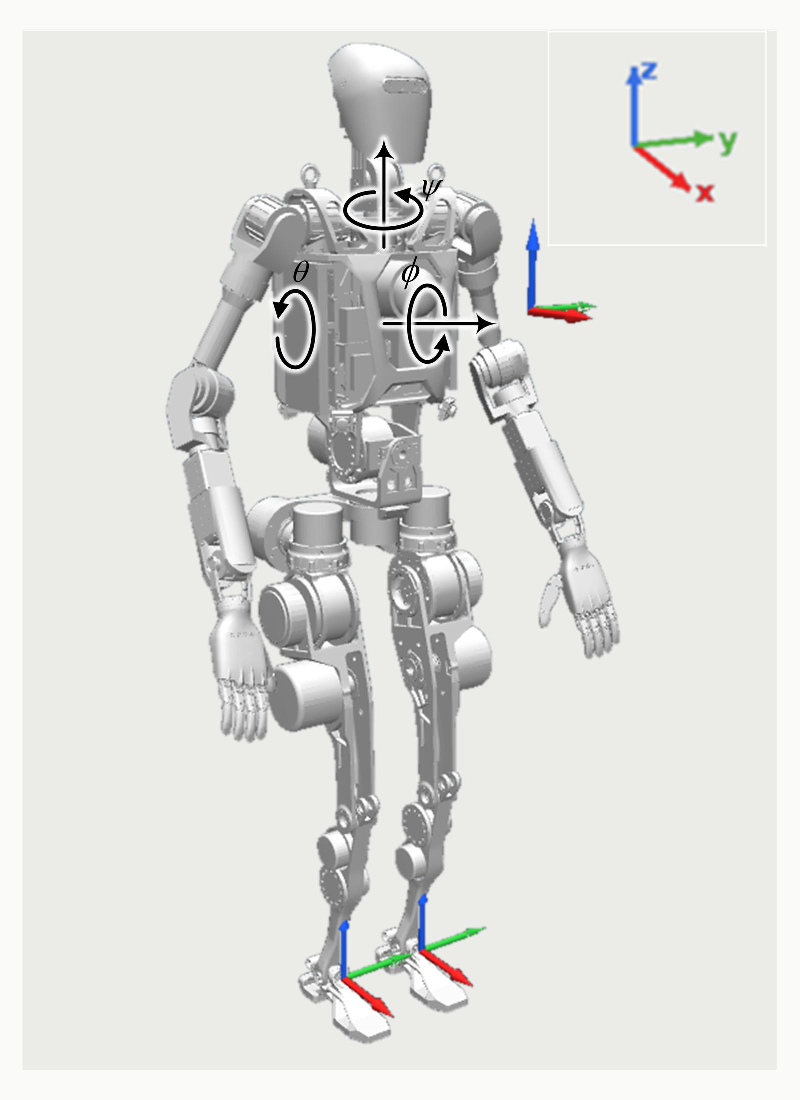
\includegraphics[height=7.2cm]{figures/manuscript_current/fig1_sign_conventions.pdf}
\caption{World-frame directions, base attitude symbols, and foot contact-force directions used in the centroidal model.}
\label{fig:sign_conventions}
\end{figure}
The SRBM adopts the following low-dimensional dynamic approximation:
\begin{equation}
m\ddot{\bm c}=\sum_{k=1}^{N_c}\bm f_k+m\bm g,
\label{eq:srbm_lin}
\end{equation}
\begin{equation}
\dot{\bm h}_G=\sum_{k=1}^{N_c}(\bm p_k-\bm c)\times \bm f_k+\sum_{k=1}^{N_c}\bm\tau_k,\quad
\bm h_G\simeq\bm I_0\bm\omega.
\label{eq:srbm_ang}
\end{equation}
Here, $\bm h_G$ denotes the angular momentum of the system about the CoM. Equations \eqref{eq:srbm_lin}--\eqref{eq:srbm_ang} indicate that conventional SRBM approximates the whole-body centroidal rotational inertia by a constant tensor $\bm I_0$, thereby describing the relationship between contact forces/moments and centroidal translational and rotational dynamics in a low-dimensional form suitable for high-frequency convex optimization. However, when a bipedal robot performs large-amplitude leg swing, high-speed stepping, or rapid attitude regulation, the swinging limbs change the whole-body inertia distribution, and $\bm I_0$ no longer accurately describes angular-momentum evolution.

To represent this configuration-dependent effect, this paper introduces the composite rotational inertia of the whole robot about the system CoM, denoted by $\bm I_G(\bm q)\in\mathbb{R}^{3\times3}$. According to the centroidal momentum representation, the angular momentum about the CoM can be decomposed into an inertia term associated with base angular velocity and a residual term associated with relative joint motion. Denoting this residual term by $\bm h_{\mathrm{rel}}(\bm q,\dot{\bm q}_j)$ gives
\begin{equation}
\bm h_G
=\bm I_G(\bm q)\bm\omega+\bm h_{\mathrm{rel}}(\bm q,\dot{\bm q}_j)
\simeq \bm I_G(\bm q)\bm\omega ,
\label{eq:IG}
\end{equation}
where $\dot{\bm q}_j$ denotes joint velocities. The low-dimensional MPC state used in this paper includes only base attitude, CoM position, base angular velocity, and CoM linear velocity; it does not explicitly predict future joint velocities or relative swing-leg motion. Therefore, $\bm h_{\mathrm{rel}}$ and its time derivative are neglected in the prediction model, leading to the approximation in \eqref{eq:IG}. This approximation retains the mass-distribution effect reflected by the configuration-dependent inertia $\bm I_G(\bm q)$.

Computationally, $\bm I_G(\bm q)$ is obtained online using the centroidal composite rigid-body algorithm. This algorithm recursively aggregates the rigid-body inertias of all branches along the robot tree to efficiently compute the whole-body inertia and CoM-related quantities \cite{ref44,ref80}. In addition to this recursive algorithm, the same centroidal inertia can also be obtained through conventional rigid-body inertia accumulation or Jacobian-based kinetic-energy equivalence. Because $\bm I_G(\bm q)$ is updated with the current configuration, it explicitly reflects the influence of swing-limb motion on the whole-body inertia distribution. Let the total moment generated by external contact wrenches about the CoM be
\begin{equation}
\bm\tau_{\text{ext}}
=\sum_{k=1}^{N_c}(\bm p_k-\bm c)\times \bm f_k+\sum_{k=1}^{N_c}\bm\tau_k .
\label{eq:tau_ext}
\end{equation}
The quantity $\bm\tau_{\text{ext}}$ in \eqref{eq:tau_ext} has the same meaning as the right-hand side of the SRBM angular equation \eqref{eq:srbm_ang}; both represent the total moment generated by all external contact wrenches about the system CoM. Specifically, $(\bm p_k-\bm c)\times \bm f_k$ is the moment of the $k$th contact force about the CoM, and $\bm\tau_k$ is the direct contact moment at that contact point. The notation $\bm\tau_{\text{ext}}$ is introduced only for compactness and does not denote an additional control input.

Using the angular-momentum balance relation $\dot{\bm h}_G=\bm\tau_{\text{ext}}$ and differentiating the low-dimensional approximate angular momentum in \eqref{eq:IG} yields
\begin{equation}
\bm\tau_{\text{ext}}
=\dot{\bm h}_G
\simeq
\bm I_G(\bm q)\dot{\bm\omega}
+\dot{\bm I}_G\bm\omega .
\label{eq:hGdot}
\end{equation}
The term $\dot{\bm I}_G\bm\omega$ denotes the angular-momentum variation induced by configuration-dependent inertia changes. Equation \eqref{eq:hGdot} is still an approximation for the low-dimensional prediction model; the omitted terms mainly come from $\dot{\bm h}_{\mathrm{rel}}$ and from relative swing-leg dynamics not explicitly modeled over the prediction horizon. The resulting angular-velocity dynamics are approximated by
\begin{equation}
\dot{\bm\omega}
\simeq
\bm I_G^{-1}\bm\tau_{\text{ext}}
-\bm I_G^{-1}\dot{\bm I}_G\bm\omega .
\label{eq:ang_dyn}
\end{equation}
Compared with conventional SRBM, the key change in \eqref{eq:ang_dyn} is that the rotational inertia used by the prediction model is no longer fixed but updated online with the joint configuration. Meanwhile, the inertia-variation term enters the local prediction model as a linear term in the angular-velocity state. To maintain consistency with force/moment-driven MPC, the state and input vectors are defined as
\begin{equation}
\begin{aligned}
\bm x&=\begin{bmatrix}\bm\Theta^\top&\bm c^\top&\bm\omega^\top&\bm v^\top\end{bmatrix}^\top,\\
\bm u&=\begin{bmatrix}\bm f_l^\top&\bm\tau_l^\top&\bm f_r^\top&\bm\tau_r^\top\end{bmatrix}^\top,
\quad \bm v=\dot{\bm c}.
\end{aligned}
\label{eq:state_input}
\end{equation}
\begin{figure*}[t]
\centering
\begin{minipage}[t]{0.48\linewidth}
\centering
\figplaceholder{figures/manuscript_current/fig1b_srbm_definition.pdf}{0.98\linewidth}{5.8cm}
\par\vspace{1mm}
{\small (a)}
\end{minipage}\hfill
\begin{minipage}[t]{0.48\linewidth}
\centering
\figplaceholder{figures/manuscript_current/fig1c_vicm_definition.pdf}{0.98\linewidth}{5.8cm}
\par\vspace{1mm}
{\small (b)}
\end{minipage}
\caption{Conceptual comparison between SRBM and VICM: (a) SRBM approximates the robot as a single rigid body with constant centroidal inertia and a small-leg-inertia assumption; (b) VICM updates the configuration-dependent centroidal inertia online and represents the inertia variation induced by leg motion within the centroidal prediction model.}
\label{fig:model_concepts}
\end{figure*}
Here, $\bm\Theta=[\phi,\theta,\psi]^\top$ denotes the base attitude angles, and $\bm f_l,\bm f_r$ and $\bm\tau_l,\bm\tau_r$ are the left- and right-foot contact forces and contact moments, respectively. Their relation to the generic contact force $\bm f_k$ and contact moment $\bm\tau_k$ in \eqref{eq:srbm_lin}--\eqref{eq:srbm_ang} is
\begin{equation}
(\bm p_1,\bm f_1,\bm\tau_1)=(\bm p_l,\bm f_l,\bm\tau_l),\qquad
(\bm p_2,\bm f_2,\bm\tau_2)=(\bm p_r,\bm f_r,\bm\tau_r).
\label{eq:contact_lr_mapping}
\end{equation}
Thus, \eqref{eq:state_input} simply expands the contact terms in \eqref{eq:srbm_lin}--\eqref{eq:srbm_ang} into MPC inputs ordered by left and right feet. When one foot is in swing phase, the corresponding contact force and contact moment are constrained to zero by the contact schedule. To clarify the origin of the prediction matrices, define
\begin{equation}
\bm r_i=\bm p_i-\bm c,\qquad
\bm S(\bm r_i)\bm f_i=\bm r_i\times\bm f_i,\quad i\in\{l,r\},
\label{eq:ri_skew}
\end{equation}
where $\bm S(\cdot)$ denotes the skew-symmetric cross-product matrix. Considering CoM translational dynamics, attitude kinematics, and the angular dynamics in \eqref{eq:ang_dyn}, and locally linearizing around the current attitude, contact geometry, and configuration-dependent inertia, one obtains
\begin{equation}
\begin{aligned}
\dot{\bm\Theta}&\simeq \bm R_z^\top\bm\omega,\\
\dot{\bm c}&=\bm v,\\
\dot{\bm\omega}
&\simeq\bm I_G^{-1}\!\left[
\bm S(\bm r_l)\bm f_l+\bm\tau_l
+\bm S(\bm r_r)\bm f_r+\bm\tau_r
\right]
-\bm I_G^{-1}\dot{\bm I}_G\bm\omega,\\
\dot{\bm v}&=\frac{1}{m}(\bm f_l+\bm f_r)+\bm g .
\end{aligned}
\label{eq:continuous_blocks}
\end{equation}
The first line of \eqref{eq:continuous_blocks} uses a yaw-only small-roll/pitch approximation to map the world-frame base angular velocity to roll-pitch-yaw rates. Under this approximation, roll and pitch rates are retained through the horizontal components of $\bm R_z^\top\bm\omega$, while higher-order roll-pitch coupling terms are omitted. Equation \eqref{eq:continuous_blocks} writes attitude kinematics, CoM translational dynamics, and centroidal angular dynamics in block form as functions of the state, contact wrench, and affine term. Arranging the terms according to the state and input order in \eqref{eq:state_input} gives the continuous-time affine model
\begin{equation}
\dot{\bm x}=\bm A_c\bm x+\bm B_c(\bm q)\bm u+\bm g_c(\bm q,\dot{\bm q}),
\label{eq:affine}
\end{equation}
with the block form
\begin{equation}
\bm A_c=
\begin{bmatrix}
\bm 0 & \bm 0 & \bm R_z^\top & \bm 0\\
\bm 0 & \bm 0 & \bm 0 & \bm I\\
\bm 0 & \bm 0 & -\bm I_G^{-1}\dot{\bm I}_G & \bm 0\\
\bm 0 & \bm 0 & \bm 0 & \bm 0
\end{bmatrix},
\label{eq:Ac}
\end{equation}
\begin{equation}
\bm B_c=
\begin{bmatrix}
\bm 0 & \bm 0 & \bm 0 & \bm 0\\
\bm 0 & \bm 0 & \bm 0 & \bm 0\\
\bm I_G^{-1}\bm S(\bm r_l) & \bm I_G^{-1} & \bm I_G^{-1}\bm S(\bm r_r) & \bm I_G^{-1}\\
\frac{1}{m}\bm I & \bm 0 & \frac{1}{m}\bm I & \bm 0
\end{bmatrix},
\label{eq:Bc}
\end{equation}
\begin{equation}
\bm g_c=
\begin{bmatrix}
\bm 0\\ \bm 0\\ \bm 0\\ \bm g
\end{bmatrix}.
\label{eq:gc}
\end{equation}
Here, $\bm R_z(\psi)$ denotes the yaw rotation constructed from the current base yaw angle, and $\bm I$ is the three-dimensional identity matrix. Equations \eqref{eq:Ac}--\eqref{eq:gc} show that $\bm A_c$ is determined by attitude kinematics, CoM position integration, and the inertia-variation term; $\bm B_c$ is determined by the contribution of contact forces and moments to centroidal angular and linear accelerations; and $\bm g_c$ collects gravity. SRBM can be viewed as a special case of this model by setting $\bm I_G(\bm q)=\bm I_0$ and $\dot{\bm I}_G=\bm 0$. VICM, in contrast, retains the same state and input dimensions while explicitly representing swing-limb inertial effects through the online update of $\bm I_G(\bm q)$ and $\dot{\bm I}_G$. In the implementation, $\dot{\bm I}_G$ is estimated by finite differencing $\bm I_G(\bm q)$ between adjacent control cycles. Since finite differencing is sensitive to configuration measurement noise and numerical errors, a first-order low-pass filter is applied before $\dot{\bm I}_G$ is used in the MPC state matrix. This filtering is a numerical smoothing step for the inertia-derivative estimate and does not change the dynamic model form in \eqref{eq:ang_dyn}. The essential difference between SRBM and VICM in inertia modeling is summarized in Fig.~\ref{fig:model_concepts}. This provides a unified dynamic basis for constructing an MPC problem that balances real-time solvability and model fidelity.

\section{Controller Design}
This section describes the closed-loop controller built on the low-dimensional centroidal dynamics introduced in Section 2. The locomotion stack is implemented based on the open-source OpenLoong Dynamics Control framework \cite{refOpenLoong}; this work modifies the centroidal prediction model and MPC dynamics terms within this framework. The controller consists of three components. First, MPC optimizes stance-foot contact wrenches over a finite prediction horizon. Second, the swing-leg planner generates foot-placement targets and swing-foot trajectories from the velocity command and gait phase. Third, WBC maps the high-level contact wrench and motion references to joint torques that satisfy full-body dynamics and contact constraints.

\subsection{MPC Controller Design}
This paper adopts a hierarchical architecture consisting of high-level centroidal MPC and low-level WBC. The high-level controller optimizes contact forces and contact moments over a finite prediction horizon based on the variable-inertia centroidal model established in Section 2. The low-level controller maps these high-level decisions to executable joint accelerations and joint torques under full-body dynamics and contact constraints. Following common receding-horizon treatments in centroidal MPC, the state and input mappings of the continuous-time model are discretized with the MPC sampling period $\Delta t_{\mathrm{mpc}}$. Because the control period is short, forward Euler discretization is adopted:
\begin{equation}
\begin{aligned}
\bm A_k&=\bm I+\Delta t_{\mathrm{mpc}}\bm A_c(k),\\
\bm B_k&=\Delta t_{\mathrm{mpc}}\bm B_c(k),\\
\bm c_k&=\Delta t_{\mathrm{mpc}}\bm c_c(k),
\end{aligned}
\label{eq:euler_disc}
\end{equation}
where $\bm A_c(k)$ and $\bm B_c(k)$ denote the continuous-time system and input matrices linearized at the $k$th prediction node using the current attitude, contact geometry, and configuration-dependent inertia, and $\bm c_c(k)$ denotes the remaining affine bias retained in the implementation. The resulting discrete-time prediction model is
\begin{equation}
\bm x_{k+1}=\bm A_k\bm x_k+\bm B_k\bm u_k+\bm c_k.
\label{eq:disc}
\end{equation}
Here, $N_p$ denotes the number of discrete predicted state nodes, so the physical prediction duration is $T_p=N_p\Delta t_{\mathrm{mpc}}$; $N_u$ denotes the control-horizon length. In the implementation, $N_u<N_p$, and the last optimized input block is held constant in the prediction matrix after the control horizon. At each control cycle, MPC solves for the optimal contact-wrench sequence $\{\bm u_0^\ast,\bm u_1^\ast,\ldots,\bm u_{N_u-1}^\ast\}$ based on the measured current state $\bm x_0$. Only the first control input $\bm u_0^\ast$ is applied, after which the horizon shifts forward by one sampling period and the optimization problem is reconstructed using the updated state. This receding-horizon mechanism continuously corrects model errors, state drift, and the influence of external disturbances. MPC minimizes state-tracking and control-regularization terms:
\begin{equation}
\scalebox{0.88}{$\displaystyle
\min_{\bm U} J=\sum_{k=1}^{N_p}\|\bm x_k-\bm x_k^{\text{ref}}\|_{\bm Q}^2+
\alpha\sum_{j=0}^{N_u-1}\|\bm u_j-\bar{\bm u}_j\|_{\bm R}^2
$}
\label{eq:cost}
\end{equation}
Here, $\bm x_k^{\text{ref}}$ is the reference trajectory for the CoM, base attitude, and angular velocity, $\bar{\bm u}_j$ is a nominal contact-wrench regularization center, $\bm Q$ and $\bm R$ are the state and input weighting matrices, respectively, and $\alpha$ is the input regularization coefficient. The nominal contact-wrench center $\bar{\bm u}_j$ provides the load-distribution reference for input regularization. In the implementation, nominal gravity-load distribution is represented by this regularization center, and the remaining affine bias in the discrete prediction model is denoted by $\bm c_k$. At the $j$th control node, it is set as
\begin{equation}
\begin{aligned}
&\bar{\bm u}_j=
\begin{bmatrix}
\bar{\bm f}_{l,j}^{\top}&\bm 0_3^{\top}&
\bar{\bm f}_{r,j}^{\top}&\bm 0_3^{\top}
\end{bmatrix}^{\top},
\\
&\bar{\bm f}_{l,j}=
-\gamma_{l,j}m\bm g,
\\
&\bar{\bm f}_{r,j}=
-\gamma_{r,j}m\bm g,
\end{aligned}
\label{eq:nominal_wrench}
\end{equation}
where $(\gamma_{l,j},\gamma_{r,j})$ is determined by the gait phase: $(1,0)$ for left support, $(0,1)$ for right support, and $(1/2,1/2)$ for double support. In the implementation, the support leg and gait phase supplied to MPC are updated by a gait scheduler that compares the measured vertical foot forces $F_{z,l}$ and $F_{z,r}$ with a predefined contact threshold. For compact notation, the resulting gait/contact state is denoted by $\chi_g$, which includes the current support leg, swing leg, and gait phase used by MPC and WBC. The user-level velocity commands $v_x^{\mathrm{cmd}}$, $v_y^{\mathrm{cmd}}$, and $\omega_z^{\mathrm{cmd}}$ are first processed through ramp generation, heading integration, and coordinate transformation to obtain the current desired state sample $\bm x_d(t)$, which contains the desired attitude, CoM position, angular velocity, and linear velocity. Inside MPC, the continuously generated samples $\bm x_d(t)$ are arranged into the stacked state reference over the prediction horizon through a rolling update. The contact wrench $\bm u_j$ is the MPC decision variable, while $\bar{\bm u}_j$ is set according to the gait phase and nominal gravity-load distribution.

Let $\bm r_n=\bm x_d(t_n)$ denote the current desired state sample generated at the $n$th MPC update. The controller maintains the stacked reference vector
\begin{equation}
\bm X_d^{(n)}
=
\begin{bmatrix}
(\bm x_{1}^{\text{ref},(n)})^\top &
(\bm x_{2}^{\text{ref},(n)})^\top &
\cdots &
(\bm x_{N_p}^{\text{ref},(n)})^\top
\end{bmatrix}^{\top}.
\label{eq:rolling_ref}
\end{equation}
At each update, this vector is shifted forward by one node and the newest reference sample $\bm r_n$ is appended to the terminal node:
\begin{equation}
\bm X_d^{(n)}
=
\begin{bmatrix}
(\bm x_{2}^{\text{ref},(n-1)})^\top &
\cdots &
(\bm x_{N_p}^{\text{ref},(n-1)})^\top &
\bm r_n^\top
\end{bmatrix}^{\top}.
\label{eq:rolling_ref_update}
\end{equation}
Therefore, $\bm x_k^{\text{ref}}$ in the cost function denotes the $k$th state-reference block in $\bm X_d$. Stacking the predicted states and inputs along the time axis as
\begin{equation}
\begin{aligned}
\bm X=
\begin{bmatrix}\bm x_1^\top&\bm x_2^\top&\cdots&\bm x_{N_p}^\top\end{bmatrix}^\top,\\
\bm U=
\begin{bmatrix}\bm u_0^\top&\bm u_1^\top&\cdots&\bm u_{N_u-1}^\top\end{bmatrix}^\top.
\end{aligned}
\label{eq:stack}
\end{equation}
the model in \eqref{eq:disc} can be written in the compact full-horizon form
\begin{equation}
\bm X=\bar{\bm A}\bm x_0+\bar{\bm B}\bm U+\bar{\bm C},
\label{eq:predcompact}
\end{equation}
where $\bar{\bm A}$, $\bar{\bm B}$, and $\bar{\bm C}$ are the stacked state-transition matrix, input-mapping matrix, and affine vector obtained recursively from the discrete-time system matrices, and $\bm x_0$ is the measured current state. To show the conversion from \eqref{eq:cost} to the quadratic program, define
\begin{equation}
\begin{aligned}
\bm X_d&=\begin{bmatrix}(\bm x_1^{\text{ref}})^\top&\cdots&(\bm x_{N_p}^{\text{ref}})^\top\end{bmatrix}^{\top},\\
\bar{\bm U}&=\begin{bmatrix}\bar{\bm u}_0^\top&\cdots&\bar{\bm u}_{N_u-1}^\top\end{bmatrix}^{\top},
\end{aligned}
\label{eq:stacked_ref_input}
\end{equation}
and let $\bar{\bm Q}=\mathrm{diag}(\bm Q,\ldots,\bm Q)$ and $\bar{\bm R}=\mathrm{diag}(\bm R,\ldots,\bm R)$. Equation \eqref{eq:cost} can then be written as
\begin{equation}
J=(\bm X-\bm X_d)^\top\bar{\bm Q}(\bm X-\bm X_d)
+\alpha(\bm U-\bar{\bm U})^\top\bar{\bm R}(\bm U-\bar{\bm U}).
\label{eq:stacked_cost}
\end{equation}
Substituting \eqref{eq:predcompact} and defining $\bm e_0=\bar{\bm A}\bm x_0+\bar{\bm C}-\bm X_d$ gives
\begin{equation}
\scalebox{0.88}{$
J=\bm U^\top(\bar{\bm B}^\top\bar{\bm Q}\bar{\bm B}+\alpha\bar{\bm R})\bm U
+2(\bar{\bm B}^\top\bar{\bm Q}\bm e_0-\alpha\bar{\bm R}\bar{\bm U})^\top\bm U.
$}
\label{eq:expanded_cost}
\end{equation}
Rearranging the result yields the standard quadratic program
\begin{equation}
\begin{aligned}
\min_{\bm U}\quad
&\frac{1}{2}\bm U^\top \bm H\bm U+\bm c^\top\bm U\\
\mathrm{s.t.}\quad
&\bm A_{\text{ineq}}\bm U\le \bm b_{\text{ineq}},\\
&\bm U_{\min}\le \bm U\le \bm U_{\max},
\end{aligned}
\label{eq:qpcompact}
\end{equation}
where $\bm H=2(\bar{\bm B}^\top\bar{\bm Q}\bar{\bm B}+\alpha\bar{\bm R})$ is the positive semidefinite Hessian induced by the weighting matrices, and $\bm c=2(\bar{\bm B}^\top\bar{\bm Q}\bm e_0-\alpha\bar{\bm R}\bar{\bm U})$ is the linear term associated with the reference trajectory, current state, and nominal contact wrench. This quadratic program imposes contact-wrench feasibility and gait-phase constraints at each prediction node. For each foot in stance phase, the linearized friction-cone constraints are
\begin{equation}
|f_{x,i}|\le \mu f_{z,i},\qquad |f_{y,i}|\le \mu f_{z,i}.
\label{eq:c_fric}
\end{equation}
Here, $f_x$, $f_y$, and $f_z$ denote the tangential and normal force components in the local foot frame, and $\mu$ is the friction coefficient. The unilateral contact condition further requires
\begin{equation}
f_{z,\min}\le f_{z,i}\le f_{z,\max}.
\label{eq:c_normal}
\end{equation}
To keep the center of pressure inside the support polygon, the foot contact moments must satisfy
\begin{equation}
-d_y^- f_{z,i}\le \tau_{x,i}\le d_y^+ f_{z,i},
\label{eq:c_copx}
\end{equation}
\begin{equation}
-d_x^- f_{z,i}\le \tau_{y,i}\le d_x^+ f_{z,i}.
\label{eq:c_copy}
\end{equation}
Here, $\tau_x$ and $\tau_y$ are the contact-moment components in the local foot frame, and $d_x^\pm$ and $d_y^\pm$ denote the geometric distances from the foot center to the support boundaries. The optimization variables also satisfy input bounds:
\begin{equation}
\bm u_{\min}\le \bm u_k\le \bm u_{\max}.
\label{eq:c_bound}
\end{equation}
For a swing foot in single-stance phase, zero-contact equality constraints are imposed:
\begin{equation}
\bm f_{\text{sw},k}=\bm 0,\qquad \bm\tau_{\text{sw},k}=\bm 0.
\label{eq:c_swing}
\end{equation}
The subscript $i$ denotes a uniformly indexed contact-wrench variable component over the prediction horizon, $k$ denotes the discrete time index, and $\text{sw}$ denotes the swing foot. Expanding \eqref{eq:c_fric}--\eqref{eq:c_swing} over the prediction horizon gives the linear inequalities and bound constraints in \eqref{eq:qpcompact}. The first optimal contact wrench obtained from the solution is sent to the low-level WBC for execution in the current control cycle.

\subsection{Swing Leg Trajectory Generation}
While MPC mainly computes stance-foot wrench distribution, the swing-foot trajectory is generated by an independent gait-planning module. Similar to the classical Raibert legged-control idea and subsequent bipedal gait-planning studies \cite{ref63,ref79}, this paper adopts a two-stage structure consisting of Raibert-type foot placement and cycloidal interpolation. The former determines the horizontal landing location from the user velocity commands, current CoM velocity, and gait phase, whereas the latter generates a swing trajectory with continuous velocity at lift-off and touchdown. The Raibert-type foot placement is
\begin{equation}
\bm p_{\text{des}}
=\bm p_{\text{hip}}
-\bm K_v(\bm v_{xy}^{\mathrm{cmd}}-\bm v_{xy})
+\frac{T_{\text{sw}}}{2}\bm v_{xy}
+(1-\phi)T_{\text{sw}}\bm v_{xy}.
\label{eq:raibert}
\end{equation}
Here, $\bm p_{\text{des}}$ is the desired landing position, $\bm p_{\text{hip}}$ is the projected hip position, $\bm v_{xy}$ is the horizontal component of the CoM velocity $\bm v$ in the state vector, $\bm v_{xy}^{\mathrm{cmd}}=[v_x^{\mathrm{cmd}},\,v_y^{\mathrm{cmd}},\,0]^\top$ is formed from the user-level horizontal velocity commands, $\bm K_v$ is the velocity-feedback gain matrix, $T_{\text{sw}}$ is the swing duration, and $\phi$ is the swing-phase variable. In the implementation, only the horizontal velocity error is used for Raibert foot placement, and the gain matrix is
\begin{equation}
\bm K_v
=\bm R_z(\psi)
\begin{bmatrix}
k_{p,v_x} & 0 & 0\\
0 & k_{p,v_y} & 0\\
0 & 0 & 0
\end{bmatrix}
\bm R_z^\top(\psi),
\label{eq:swing_kv}
\end{equation}
where $\psi$ is the current base yaw angle and $\bm R_z(\psi)$ maps the horizontal feedback gains from the body-aligned frame to the world frame. The scalar gains $k_{p,v_x}$ and $k_{p,v_y}$ are listed in Table~\ref{tab:swing_param}. For turning gaits, an additional yaw correction is introduced:
\begin{equation}
\Delta \bm p_{\text{yaw}}
=\frac{w_{\text{hip}}}{2}
\begin{bmatrix}
\cos\theta_f-\cos\theta_0\\
\sin\theta_f-\sin\theta_0\\
0
\end{bmatrix},
\end{equation}
\begin{equation}
\theta_f=\theta_0+\omega_z(1-\phi)T_{\text{sw}}+\frac{1}{2}\omega_zT_{\text{sw}}+k_{p,\omega_z}(\omega_z-\omega_z^{\mathrm{cmd}}).
\label{eq:yaw}
\end{equation}
Here, $w_{\text{hip}}$ is the lateral hip distance, $\theta_0$ and $\theta_f$ are the current and predicted yaw angles, $\omega_z$ is the yaw component of the angular velocity $\bm\omega$ in the state vector, $\omega_z^{\mathrm{cmd}}$ is the user-level yaw-rate command, and $k_{p,\omega_z}$ is the yaw-feedback gain. Given the landing point, the swing-phase interpolation function is
\begin{equation}
s(\phi)=\phi-\frac{\sin(2\pi\phi)}{2\pi}.
\label{eq:phase}
\end{equation}
The horizontal and vertical swing trajectories are then
\begin{equation}
\bm p_{xy}^{\text{sw}}(\phi)=\bm p_{xy}^{0}+s(\phi)\left(\bm p_{xy}^{f}-\bm p_{xy}^{0}\right),
\label{eq:trajxy}
\end{equation}
\begin{equation}
z^{\text{sw}}(\phi)=z_0+\frac{h}{2}\left(1-\cos 2\pi\phi\right)+s(\phi)(z_f-z_0).
\label{eq:trajz}
\end{equation}
In \eqref{eq:trajz}, $h$ is the swing-foot clearance height $H_{\mathrm{step}}$. The terminal foot height is generated from the nominal standing leg length and the foot-height compensation used in the controller, so that the planned foot endpoint remains consistent with the desired base height during flat-ground walking. This planning method maintains velocity continuity at lift-off and touchdown and reduces impact during contact transitions.

\begin{table}[t]
\centering
\caption{Main swing-leg planning parameters}
\label{tab:swing_param}
\scriptsize
\begin{tabular*}{\linewidth}{@{\extracolsep{\fill}}L{0.43\linewidth}L{0.20\linewidth}L{0.27\linewidth}@{}}
\hline
Parameter & Symbol/unit & Value \\
\hline
Velocity feedback gain in $x$ direction & $k_{p,v_x}$ & 0.10 \\
Velocity feedback gain in $y$ direction & $k_{p,v_y}$ & 0.03 \\
Yaw feedback gain & $k_{p,\omega_z}$ & 0.03 \\
Swing duration & $T_{\mathrm{sw}}$/s & 0.45 (Exp. 1, 3, 4) \\
 & & 0.25 (Exp. 2) \\
Swing-foot clearance height & $H_{\mathrm{step}}$/m & 0.205 \\
Foot-height compensation & $h_{\mathrm{foot}}$/m & 0.07 \\
Nominal standing leg length & $L_{\mathrm{leg}}$/m & 1.05 \\
Lateral hip distance & $w_{\mathrm{hip}}$/m & 0.209 \\
\hline
\end{tabular*}
\end{table}

\subsection{WBC Controller Design}
The WBC layer follows a widely used low-level implementation combining centroidal MPC with an inverse-dynamics QP \cite{ref36,ref55,ref63}. It recovers full-body dynamic feasibility at the high-frequency control layer, enforces contact consistency, and executes swing-leg and torso tasks. The basic dynamic constraints are
\begin{equation}
\bm M(\bm q)\ddot{\bm q}
+\bm C(\bm q,\dot{\bm q})\dot{\bm q}
+\bm G(\bm q)
=\bm S^\top\bm\tau_j+\bm J_c^\top\bm f,
\label{eq:wbcdyn}
\end{equation}
\begin{equation}
\bm J_c\ddot{\bm q}+\dot{\bm J}_c\dot{\bm q}=\bm 0.
\label{eq:wbccontact}
\end{equation}
Equation \eqref{eq:wbcdyn} gives the full-body inverse-dynamics balance, and \eqref{eq:wbccontact} enforces rigid-contact acceleration constraints at stance contacts. The left- and right-foot contact forces $\bm f_l,\bm f_r$ provided by high-level MPC and the desired generalized acceleration $\ddot{\bm q}_{\text{ref}}$ generated by the task layer from stance-contact, torso-regulation, and swing-foot tracking tasks jointly form the WBC reference input. Based on this reference input, the low-level inverse-dynamics QP solves for the minimum correction satisfying \eqref{eq:wbcdyn}, \eqref{eq:wbccontact}, and the feasible contact-force set:
\begin{equation}
\min_{\delta\ddot{\bm q},\delta\bm f,\bm\tau_j}
\left\|\delta\ddot{\bm q}\right\|^2
+\left\|\delta\bm f\right\|^2
+\left\|\bm\tau_j\right\|^2
\label{eq:wbcqp}
\end{equation}
subject to
\begin{equation}
\ddot{\bm q}=\ddot{\bm q}_{\text{ref}}+\delta\ddot{\bm q},\qquad
\bm f=\begin{bmatrix}\bm f_l^\top&\bm f_r^\top\end{bmatrix}^\top+\delta\bm f,
\end{equation}
\begin{equation}
\bm\tau_{j,\min}\le \bm\tau_j\le \bm\tau_{j,\max},\qquad \bm f\in\mathcal{K}_\mu.
\label{eq:wbcbound}
\end{equation}
The variables $\delta\ddot{\bm q}$ and $\delta\bm f$ are the corrections to the reference acceleration and reference contact force, respectively, and $\mathcal{K}_\mu$ denotes the feasible set of the linearized friction cone. Based on the desired contact wrench from high-level MPC and the motion references generated by the task layer, the low-level WBC jointly solves for the generalized acceleration $\ddot{\bm q}$, contact force $\bm f$, and joint torque $\bm\tau_j$ that satisfy dynamics and contact constraints. In the implementation, the WBC output is converted into the joint position reference $\bm q^{\mathrm{des}}$, joint velocity reference $\dot{\bm q}^{\mathrm{des}}$, and joint-torque feedforward $\bm\tau_j^{\mathrm{ff}}$ for a joint-level Position-Velocity-Torque (PVT) controller, which then generates the final motor torque $\bm\tau^{\mathrm{out}}$ for the simulated robot. WBC tasks include stance-contact consistency, torso attitude and position regulation, swing-leg trajectory tracking, and regulation of the upper limbs and redundant joints. Since this paper focuses on the difference between high-level prediction models, the WBC task structure and parameters are kept identical in all comparative experiments and serve as a unified full-body dynamic execution layer. The information flow among MPC, swing-leg planning, WBC, and the robot plant is summarized in Fig.~\ref{fig:control_framework}, where user velocity commands are converted into references for MPC and foot placement, and the optimized contact wrench together with task-level motion references forms the WBC input.
\begin{figure}[t]
\centering
\figplaceholder{figures/manuscript_current/fig3.jpg}{0.88\linewidth}{5.3cm}
\caption{Overall control framework.}
\label{fig:control_framework}
\end{figure}

\section{Simulation and Performance Comparison}
This section evaluates the proposed VICM-MPC and the SRBM-MPC baseline in MuJoCo full-body dynamics simulation. The simulation setup, robot parameters, and unified controller parameters are first specified. Four experiments are then designed, including leg-inertia sweeping, nominal velocity tracking, model-structure ablation, and external disturbance recovery. The results are compared in terms of survival time, tracking response, ablation behavior, disturbance-recovery region, and online computation time.

\subsection{Simulation Setup and Robot Parameters}
All comparative experiments are conducted in the MuJoCo full-body dynamics simulation platform. Pinocchio is used for kinematic and dynamic computations, ensuring consistency among simulated state feedback, contact information, and the internal model used by the controller. Representative walking snapshots from the simulation environment are shown in Fig.~\ref{fig:walking_snapshots}. The main simulation parameters corresponding to the control code are listed in Table~\ref{tab:sim_param}.

\begin{figure*}[t]
\centering
\figplaceholder{figures/manuscript_current/fig4_walking_snapshots.png}{0.86\linewidth}{5.2cm}
\caption{Side-view walking snapshots of the robot on flat ground. The first three frames are sampled during the startup double-support interval, and the remaining frames show the subsequent single-support walking motion. The labels indicate double-, left-, and right-support phases, and the white dashed vertical lines mark support-phase transitions.}
\label{fig:walking_snapshots}
\end{figure*}

\begin{table*}[t]
\centering
\caption{Main simulation parameters}
\label{tab:sim_param}
\begin{tabular*}{\linewidth}{@{\extracolsep{\fill}}lcc}
\hline
Parameter & Symbol/unit & Value \\
\hline
Simulator & -- & MuJoCo \\
Kinematics/dynamics library & -- & Pinocchio \\
Dynamics integration step & $\Delta t_{\mathrm{sim}}$/s & 0.001 \\
WBC update period & $\Delta t_{\mathrm{wbc}}$/s & 0.001 \\
MPC update period & $\Delta t_{\mathrm{mpc}}$/s & 0.005 \\
Gravitational acceleration & $\bm g$/m$\cdot$s$^{-2}$ & $[0,0,-9.81]^\top$ \\
Prediction horizon length & $N_p$ & 10 \\
Effective prediction time & $N_p\Delta t_{\mathrm{mpc}}$/s & 0.05 \\
Control horizon length & $N_u$ & 3 \\
Ground friction coefficient & $\mu$ & 0.5 \\
Maximum simulation time & $T_{\mathrm{sim}}$/s & 30 \\
\hline
\end{tabular*}
\end{table*}

The quantities $\bm I_G(\bm q)$ and $\dot{\bm I}_G$ used over the prediction horizon are locally linearized at the measured configuration of the current control cycle and recomputed at the next cycle under the receding-horizon mechanism. With $N_p=10$, the effective prediction time is 0.05 s.

The tested robot is the full-body AzureLoong model. Its mass parameters, inertial parameters, and joint layout are consistent with the URDF model used by the control code, and the reported geometric dimensions are extracted from the MJCF/URDF model used in simulation. Table~\ref{tab:robot_param} lists the main robot parameters used in the simulation model.

\begin{table}[t]
\centering
\caption{Main robot parameters}
\label{tab:robot_param}
\scriptsize
\begin{tabular*}{\linewidth}{@{\extracolsep{\fill}}L{0.36\linewidth}L{0.23\linewidth}L{0.31\linewidth}@{}}
\hline
Parameter & Symbol/unit & Value \\
\hline
Robot model & -- & AzureLoong full-body model \\
Total mass & $m$/kg & 77.35 \\
Body/non-leg mass & $M_b^0$/kg & 47.48 \\
Bilateral leg mass & $M_\ell^0$/kg & 29.87 \\
Standing height from MJCF geometry & $H$/m & 1.818 \\
Base-link bounding-box size & $l_b,w_b,h_b$/m & 0.297, 0.327, 0.540 \\
Nominal standing base height & $H_b$/m & 1.12 \\
Hip-to-knee and knee-to-ankle offsets & $l_1,l_2$/m & 0.400, 0.387 \\
Foot collision-box size & $l_f,w_f,h_f$/m & 0.245, 0.080, 0.088 \\
Base-link inertia in URDF & $(I_{xx},I_{yy},I_{zz})$/kg\,m$^2$ & 0.374, 0.277, 0.221 \\
Number of URDF links & -- & 32 \\
Number of URDF joints & -- & 31 \\
\hline
\end{tabular*}
\end{table}

The following MPC weighting matrices are used in simulation:
\begin{equation}
\bm Q=\mathrm{diag}(50,50,80,\,1,200,1,\,1,1,10,\,100,10,1),
\end{equation}
\begin{equation}
\bm R=\bm I_{13},
\end{equation}
with input regularization coefficient $\alpha=10^{-6}$. The matrix $\bm Q$ corresponds to the diagonal weights of the state vector in \eqref{eq:state_input}, acting on base attitude, CoM position, angular velocity, and CoM linear velocity, respectively. The matrix $\bm R$ corresponds to the diagonal weights of the contact-wrench input vector. Across all experiments, MPC weights, MPC constraints, WBC parameters, gait scheduling parameters, and swing-leg planning parameters are kept unchanged.

\subsection{Experimental Design}
Four sets of comparative experiments are designed. The core comparison is between a controller based on the constant-inertia single rigid body model (SRBM-MPC) and a controller based on the variable-inertia centroidal model with configuration-dependent inertia and inertia-variation terms (VICM-MPC). Unless otherwise stated, all controllers share the same MPC weights, MPC constraints, WBC execution layer, WBC parameter settings, swing-leg planner, and contact-switching settings. Gait switching uses the touchdown detection signal, with a normal contact-force threshold of 100 N. In VICM-MPC, $\dot{\bm I}_G$ is computed by finite differencing $\bm I_G$ between adjacent control cycles and then passing it through a first-order low-pass filter with a time constant of 0.01 s.

Experiment 1 analyzes the difference in stability margin between the two models as swing-leg inertia increases. Specifically, different degrees of swing-inertia perturbation are constructed by a leg mass and inertia scaling factor $\lambda$, and the same forward velocity command and sinusoidal yaw-rate command are applied at each value of $\lambda$. The values of $\lambda$ are $1.0,1.1,\ldots,2.3$, corresponding to 1.0--2.3 times the nominal leg mass and inertia, with a step size of 0.1. At each $\lambda$, SRBM-MPC and VICM-MPC are each run five times, and the maximum duration of a single simulation is 30 s. The forward velocity command is $v_x^{\mathrm{cmd}}=1.5$ m/s, and the swing duration is $T_{\mathrm{sw}}=0.45$ s. The turning command is zero for $t<4$ s and is set for $t\ge4$ s as
\begin{equation}
\omega_z^{\mathrm{cmd}}(t)=0.25\sin\left(\frac{2\pi(t-4)}{4}\right)\ \mathrm{rad/s}.
\label{eq:exp_sine_wz}
\end{equation}
The main evaluation metric is survival time, defined as the duration before falling or losing stability, and the mean and dispersion over the five repeated trials are reported. By scanning $\lambda$, the experiment reveals the sensitivity difference between SRBM and VICM to model approximation errors when swing-limb inertia increases and turning-induced angular-momentum variation becomes stronger.

The leg inertia scaling is implemented as follows. Let $\mathcal{L}$ denote the set of left- and right-leg links, including the links associated with the hips, knees, and ankles. For each leg link $i\in\mathcal{L}$, its mass and rotational inertia are scaled by the same factor $\lambda$:
\begin{equation}
m_i(\lambda)=\lambda m_i^0,\qquad
\bm I_i(\lambda)=\lambda \bm I_i^0 ,
\label{eq:leg_lambda_scaling}
\end{equation}
where the superscript 0 denotes the nominal inertial parameter in the URDF. The inertial parameters of non-leg links are kept unchanged; hence the total robot mass and leg mass fraction increase with $\lambda$. The corresponding two-leg mass fraction is
\begin{equation}
\rho_\ell(\lambda)=
\frac{\lambda M_\ell^0}{M^0+(\lambda-1)M_\ell^0},
\label{eq:leg_mass_fraction_lambda}
\end{equation}
where $M^0$ is the nominal total robot mass and $M_\ell^0$ is the nominal total mass of both legs. According to the nominal URDF mass parameters, the total robot mass is 77.35 kg and the total mass of the left and right leg links is 29.87 kg, corresponding to a nominal two-leg mass fraction of 0.386. This scaling strategy systematically examines the effect of swing-leg inertia variation on gait stability without changing the control architecture or swing-leg planner.

Experiment 2 presents velocity-tracking performance under the nominal mass distribution. This experiment uses $\lambda=1.0$, imposes no turning target, runs a single simulation for 16 s, and sets the swing duration to $T_{\mathrm{sw}}=0.25$ s. In the forward-velocity experiment, the lateral velocity command is kept at zero, the forward velocity command is 0.6 m/s for $t<8$ s, linearly ramps to 1.2 m/s over $8\le t\le11$ s, and remains at 1.2 m/s for $t>11$ s. In the lateral-velocity experiment, the forward velocity command is kept at zero, the lateral velocity command is 0.15 m/s for $t<8$ s, linearly ramps to 0.30 m/s over $8\le t\le11$ s, and remains at 0.30 m/s for $t>11$ s. Experiment 2 shows representative velocity responses of SRBM-MPC and VICM-MPC, illustrating that both low-dimensional models can be embedded in the same MPC--WBC framework when the two-leg mass fraction is low.

Experiment 3 analyzes the contribution of internal VICM modeling terms to stability. This experiment uses $\lambda=1.7$, a forward velocity command of $v_x^{\mathrm{cmd}}=1.5$ m/s, a swing duration of $T_{\mathrm{sw}}=0.45$ s, the same yaw-rate command as \eqref{eq:exp_sine_wz}, and a maximum single-run duration of 30 s. Each model variant is repeated three times. The four compared variants are defined in the order used in Fig.~\ref{fig:experiment3_ablation}. SRBM uses the constant-inertia single rigid body model. VICM denotes the complete variable-inertia centroidal model, which updates $\bm I_G(\bm q)$ online, incorporates $-\bm I_G^{-1}\dot{\bm I}_G\bm\omega$ into the angular-velocity block of the state matrix, and applies low-pass filtering to the finite-difference estimate of $\dot{\bm I}_G$. VICM-IG updates $\bm I_G(\bm q)$ online but does not use the inertia-variation term $-\bm I_G^{-1}\dot{\bm I}_G\bm\omega$. VICM-NF uses the same model form as VICM and still includes $-\bm I_G^{-1}\dot{\bm I}_G\bm\omega$, but disables the first-order low-pass filtering of the finite-difference $\dot{\bm I}_G$. This ablation study separates the effects of configuration-dependent inertia, the inertia-variation term, and numerical smoothing on closed-loop stability and angular-velocity prediction error.

Experiment 4 evaluates gait-recovery capability under external disturbances. This experiment uses $\lambda=1.7$, a forward velocity command of $v_x^{\mathrm{cmd}}=1.2$ m/s, no turning command, a swing duration of $T_{\mathrm{sw}}=0.45$ s, and a maximum simulation time of 15 s. A horizontal impulse-like disturbance is applied to the robot torso. To avoid applying the disturbance exactly at a contact-switching boundary due to a fixed absolute time, the disturbance is triggered after $t\ge8$ s when the gait phase first reaches $\phi=0.5$, and lasts 0.15 s. The disturbance direction angle $\theta_F$ takes $0^\circ,45^\circ,\ldots,315^\circ$, and the force amplitudes are $0,100,200,300,400$ N. Each direction-amplitude combination is repeated five times for both SRBM-MPC and VICM-MPC. The experiment records whether the robot maintains locomotion until the end of the simulation and plots the direction-amplitude recovery region and representative disturbance responses.

In summary, Experiment 1 statistically evaluates stability margin under different leg inertias; Experiment 2 shows nominal velocity-tracking curves; Experiment 3 provides a structural ablation of the model; and Experiment 4 presents disturbance-recovery regions and representative responses. Together, these four experiments compare the applicability boundaries of the modeling strategies under parameter perturbation, regular tracking, and external disturbance.

\subsection{Results and Comparative Analysis}
The results of Experiment 1 show that when leg inertia is nominal or moderate, both SRBM-MPC and VICM-MPC can maintain stable walking, and their difference is not pronounced. When leg inertia is further increased and a periodic turning command is imposed, SRBM-MPC approaches the hybrid stability boundary earlier, whereas VICM-MPC achieves a longer survival time in selected high-inertia cases. As shown in Fig.~\ref{fig:experiment1_leg_fraction}, the results can be divided into three regions: (a) in the nominal region, both models remain close to the 30 s simulation limit; (b) in the boundary region, VICM-MPC achieves a longer survival time at several values of $\lambda$; and (c) in the extremely high-inertia region, both controllers lose stability rapidly and the model difference diminishes as overall feasibility degrades. To provide the velocity-response background, this paper also reports the forward velocity curves for $\lambda=1.0$ and $\lambda=1.7$. As shown in Fig.~\ref{fig:experiment1_tracking}, the actual forward velocities of both controllers are below the 1.5 m/s command. During the overlapping time interval in which both controllers remain stable, SRBM-MPC and VICM-MPC exhibit comparable forward velocity levels. In the $\lambda=1.7$ case, SRBM-MPC loses stability at approximately 16.5 s, whereas VICM-MPC completes the 30 s simulation. These results show that VICM-MPC provides a larger stability margin when swing-leg inertia is high and turning-induced angular-momentum variation is pronounced, while the actual forward velocity levels of the two controllers remain comparable.

\begin{figure}[t]
\centering
\figplaceholder{figures/manuscript_current/exp1_lambda_turning_survival.png}{0.88\linewidth}{5.2cm}
\caption{Experiment 1: survival time under high-leg-inertia turning conditions. The plot is divided according to the leg-inertia scale: (a) nominal region, where the two models show a small difference; (b) boundary advantage region, where VICM-MPC achieves a longer survival time at selected high-inertia points; and (c) joint-failure region, where both controllers rapidly lose stability.}
\label{fig:experiment1_leg_fraction}
\end{figure}

The observed loss of stability does not need to occur immediately at the beginning of simulation to be attributed to the prediction model. Bipedal walking is a hybrid dynamic system with periodic contact switching. Angular-dynamics prediction errors in MPC can accumulate through stance-phase contact wrenches, torso attitude errors, effective foot-placement quality, and subsequent contact transitions. Therefore, if instability occurs after several steps and is preceded by increasing attitude or angular-velocity errors and contact-wrench allocation differences, it can still be interpreted as the amplification of low-dimensional prediction-model errors over gait cycles. Of course, if the loss of stability is strictly accompanied by swing-foot tracking failure, joint-torque saturation, or WBC infeasibility, further investigation using swing-leg tracking errors and WBC residuals is required.

\begin{figure}[t]
\centering
\figplaceholder{figures/manuscript_current/exp1_representative_tracking_body_forward.png}{0.88\linewidth}{6.8cm}
\caption{Forward velocity responses in Experiment 1, with $v_x^{\mathrm{cmd}}=1.5$ m/s, $T_{\mathrm{sw}}=0.45$ s, and the yaw-rate command given by \eqref{eq:exp_sine_wz}: (a) nominal leg-inertia case with $\lambda=1.0$; (b) high-leg-inertia case with $\lambda=1.7$.}
\label{fig:experiment1_tracking}
\end{figure}

\begin{figure}[t]
\centering
\figplaceholder{figures/manuscript_current/exp2_nominal_velocity_ramp_tracking.png}{0.88\linewidth}{5.2cm}
\caption{Experiment 2: velocity-ramp tracking under the nominal mass distribution: (a) forward walking with a ramped $v_x^{\mathrm{cmd}}$ command and $v_y^{\mathrm{cmd}}=0$; (b) lateral walking with a ramped $v_y^{\mathrm{cmd}}$ command and $v_x^{\mathrm{cmd}}=0$.}
\label{fig:experiment2_speed}
\end{figure}

Experiment 2 shows velocity-tracking results under the nominal mass distribution. Both the forward-velocity ramp experiment and the lateral-velocity ramp experiment indicate that, under nominal mass distribution and non-turning conditions, the closed-loop velocity responses of the two models are close, and VICM does not exhibit a decisive tracking advantage. This result is consistent with the main claim of this paper: with WBC, foot-placement planning, and closed-loop feedback, SRBM already performs well in regular walking tasks, and the main value of VICM lies not in universally improving nominal velocity tracking, but in improving angular-dynamics prediction consistency under boundary conditions. The corresponding velocity-tracking curves are shown in Fig.~\ref{fig:experiment2_speed}.

The ablation results of Experiment 3 show that both configuration-dependent inertia and the inertia-variation term affect closed-loop stability. Under the same high-leg-inertia and turning command, SRBM-MPC loses stability at approximately 16.7 s. VICM-IG extends survival time but still does not complete the full simulation. The complete VICM further incorporates the inertia-variation term into the angular-velocity state matrix and completes the 30 s simulation. VICM-NF exhibits stronger numerical sensitivity, indicating that moderate smoothing of $\dot{\bm I}_G$ helps suppress spike responses caused by finite differencing or configuration measurement noise. The corresponding results are shown in Fig.~\ref{fig:experiment3_ablation}.

Experiment 4 indicates that, under phase-aligned horizontal pulse disturbances, VICM-MPC has a larger recovery region for selected directions and magnitudes. The binary recovery map shows that VICM-MPC withstands higher tested push forces in directions such as $45^\circ$, $90^\circ$, $135^\circ$, and $315^\circ$, whereas SRBM-MPC performs better in the $270^\circ$ direction. The observed directional asymmetry may originate from the specific stance/swing-leg state at the push trigger, left--right contact execution differences, and phase deviations near contact switching. The corresponding binary recovery maps and recovery boundary are shown in Fig.~\ref{fig:experiment4_recovery}, where the enclosed recovery-boundary area of VICM is 1.47 times that of SRBM.

The online computation time is measured under the representative high-inertia turning condition with $\lambda=1.7$. After excluding initialization outputs, 1805 control cycles are recorded for each controller. As shown in Table~\ref{tab:mpc_timing}, both controllers keep the average wall-clock time below the 5 ms MPC update period.

\begin{figure}[t]
\centering
\figplaceholder{figures/manuscript_current/exp3_model_ablation_summary.png}{0.78\linewidth}{8.8cm}
\caption{Experiment 3: ablation analysis of the internal modeling terms in VICM. SRBM is the single rigid body model; VICM is the complete model using configuration-dependent inertia $\bm I_G(\bm q)$, the inertia-variation term $-\bm I_G^{-1}\dot{\bm I}_G\bm\omega$, and low-pass filtering of $\dot{\bm I}_G$; VICM-IG uses only configuration-dependent inertia $\bm I_G(\bm q)$; and VICM-NF includes the inertia-variation term but disables $\dot{\bm I}_G$ filtering. Panels report (a) survival time, (b) one-step angular-velocity prediction error, (c) RMS yaw-rate tracking error, and (d) maximum torso attitude error.}
\label{fig:experiment3_ablation}
\end{figure}

\begin{table}[t]
\centering
\caption{Single-step computation time comparison between SRBM-MPC and VICM-MPC}
\label{tab:mpc_timing}
\scriptsize
\begin{tabular*}{\linewidth}{@{\extracolsep{\fill}}lccccc@{}}
\hline
Controller & Samples & Mean & Max & QP mean & QP max \\
 & & [ms] & [ms] & [ms] & [ms] \\
\hline
SRBM-MPC & 1805 & 1.78 & 5.21 & 1.12 & 3.99 \\
VICM-MPC & 1805 & 1.77 & 5.37 & 1.13 & 3.67 \\
\hline
\end{tabular*}
\end{table}

Taken together, the four experiments show that SRBM remains a strong low-dimensional model when the two-leg mass fraction is low, while the benefit of VICM mainly appears when swing-leg inertia is large, turning-induced angular-momentum variation is pronounced, and the system operates near contact-switching and attitude-recovery boundaries. Under these conditions, introducing configuration-dependent inertia and its variation improves angular-dynamics prediction consistency and enlarges the stability margin in selected scenarios.

\begin{figure}[t]
\centering
\figplaceholder{figures/manuscript_current/exp4_recovery_binary_and_boundary.png}{0.78\linewidth}{8.2cm}
\caption{Experiment 4: recovery region under phase-triggered horizontal pulse disturbances. The disturbance is applied when the gait phase first reaches $\phi=0.5$ after $t\ge8$ s. The direction angle $\theta_F$ takes $0^\circ,45^\circ,\ldots,315^\circ$, the force amplitudes are $0,100,200,300,400$ N, and each combination is repeated five times. Black cells denote recovered cases that remain stable until the end of simulation, whereas white cells denote failed cases; (a) SRBM-MPC, (b) VICM-MPC, (c) maximum tested recoverable push-force boundary by direction, and (d) top-view direction convention, where $\theta_F$ is measured counterclockwise from $+X$, with $0^\circ$ along $+X$ and $90^\circ$ along $+Y$. $A_{\mathrm{VICM}}$ and $A_{\mathrm{SRBM}}$ denote the enclosed areas of the VICM and SRBM polar recovery boundaries in (c), respectively.}
\label{fig:experiment4_recovery}
\end{figure}

\section{Conclusion and Future Work}
This paper proposed a bipedal robot model predictive control method based on a variable-inertia centroidal model to address angular-dynamics prediction errors caused by the constant-inertia assumption in conventional single rigid body models. By introducing the configuration-dependent centroidal inertia tensor online and incorporating the effect of inertia variation on angular-velocity evolution into a low-dimensional prediction model, the proposed method constructs a prediction model that balances real-time efficiency and dynamic fidelity. Combined with a contact-constrained MPC formulation, Raibert foot placement, and a low-level inverse-dynamics QP execution layer, the method forms a complete hierarchical control framework.

Representative simulation results show that, compared with SRBM-MPC using a constant-inertia approximation, the proposed VICM-MPC can achieve a longer survival time and a larger empirical recovery region in selected conditions with high leg inertia, pronounced turning-induced angular-momentum variation, or transient external disturbances. At the same time, in velocity-tracking tasks with a low two-leg mass fraction, the closed-loop behavior of the two models is similar, indicating that SRBM remains highly effective when WBC, foot-placement planning, and feedback control act together. These results suggest that the value of configuration-dependent centroidal inertia and its variation mainly lies in improving angular-dynamics prediction consistency and stability margin under boundary conditions; in low-leg-inertia, non-turning regular walking tasks, the performance difference between the two models is relatively limited.

Several limitations remain. First, the current results are obtained from MuJoCo flat-ground simulations and do not yet cover real-robot execution errors, ground uncertainty, or sensor noise. Second, the low-dimensional MPC uses locally linearized inertia at the current configuration over the prediction horizon and does not explicitly predict future swing-leg configuration evolution; therefore, the advantage of VICM is still limited by receding linearization accuracy. Third, $\dot{\bm I}_G$ is currently obtained by finite differencing and low-pass filtering, and its numerical quality affects the stability of the angular-velocity state matrix. More accurate inertia-derivative computation and horizon-wise update methods should be investigated. Finally, the disturbance experiments use finite grids of directions, magnitudes, and phase-triggered timings. The asymmetry of the recovery boundary may be related to the stance-leg state, left--right contact execution differences, and contact-switching phase. Additional repeated trials, more gait conditions, and WBC execution-error analysis are needed to further separate the contributions of model error, swing-leg tracking error, and low-level torque constraints to instability.

Future work will proceed in several directions. First, the proposed method will be deployed on a physical bipedal robot to verify its real-time performance and engineering feasibility in continuous flat-ground walking, velocity transitions, and external disturbance recovery. Second, the current flat-ground contact model will be extended to uneven terrain, discrete footholds, and multi-contact scenarios to evaluate the applicability of variable-inertia modeling in more complex environments. Third, consistency enhancement between centroidal prediction models and full-body dynamics will be further studied, together with improved update strategies for configuration-dependent inertia and its time derivative over the prediction horizon. In addition, the integration of this model with reinforcement-learning control frameworks will be explored, for example by using it as a model prior, safety constraint, or residual policy structure. Finally, perception information and learning strategies will be incorporated to improve the robot's generalization and autonomy in unknown environments.

\section*{Acknowledgments}
This work was supported by the National Natural Science Foundation of China (Grant Nos. 12532002, 12372065, U2441202, 12272167) and the Open Fund Program of the National and Local Co-Build Humanoid Robotics Innovation Center (Grant No. HRCPUR20251106003).

\begin{thebibliography}{100}
\bibitem{ref22} Z. Gu, J. Li, W. Shen, et al., Humanoid locomotion and manipulation: current progress and challenges in control, planning, and learning, arXiv preprint arXiv:2501.02116 (2025).
\bibitem{ref23} M. Chignoli, D. Kim, E. Stanger-Jones, et al., The MIT humanoid robot: design, motion planning, and control for acrobatic behaviors, in: IEEE-RAS Humanoids, 2021.
\bibitem{ref20} Y. Zhao, Y. Li, L. Sentis, et al., Reactive task and motion planning for robust whole-body dynamic locomotion in constrained environments, Int. J. Robot. Res. 41(8) (2022) 812--847.
\bibitem{ref74} Z. Li, X. Zhou, S. Chen, et al., Development of a humanoid robot Wukong 4.0 for complex terrain adaptation, in: IEEE ICMA, 2022, pp. 125--130.
\bibitem{ref78} L. Han, X. Chen, Z. Yu, et al., Balance control method for underactuated biped robots on discrete terrain, Acta Automatica Sinica 48(9) (2022) 2164--2174 (in Chinese).
\bibitem{ref12} M. Vukobratovi\'{c}, B. Borovac, Zero-moment point---thirty five years of its life, Int. J. Humanoid Robot. 1(1) (2004) 157--173.
\bibitem{ref17} S. Kajita, F. Kanehiro, K. Kaneko, et al., The 3D linear inverted pendulum mode: a simple modeling for a biped walking pattern generation, in: IEEE/RSJ IROS, 2001, pp. 239--246.
\bibitem{ref18} S. Kajita, F. Kanehiro, K. Kaneko, et al., Biped walking pattern generation by using preview control of zero-moment point, in: IEEE ICRA, 2003, pp. 1620--1626.
\bibitem{ref14} A. D. Ames, Human-inspired control of bipedal walking robots, IEEE Trans. Autom. Control 59(5) (2014) 1115--1130.
\bibitem{ref16} E. R. Westervelt, J. W. Grizzle, D. E. Koditschek, Hybrid zero dynamics of planar biped walkers, IEEE Trans. Autom. Control 48(1) (2003) 42--56.
\bibitem{ref25} J. Li, Q. Nguyen, Force-and-moment-based model predictive control for achieving highly dynamic locomotion on bipedal robots, in: IEEE CDC, 2021.
\bibitem{ref36} A. Herzog, N. Rotella, S. Mason, et al., Momentum control with hierarchical inverse dynamics on a torque-controlled humanoid, Autonomous Robots 40(3) (2016) 473--491.
\bibitem{ref55} Q. Rouxel, S. Ivaldi, J.-B. Mouret, Multi-contact whole-body force control for position-controlled robots, IEEE Robot. Autom. Lett. 9(6) (2024) 5639--5646.
\bibitem{ref63} X. Wang, W. Guo, S. Yin, et al., Walking control of humanoid robots based on improved footstep planner and whole-body coordination controller, Front. Neurorobot. 19 (2025) 1538979.
\bibitem{refOpenLoong} Humanoid Robot (Shanghai) Co., Ltd, OpenLoong-DynamicsControl: Motion control framework of humanoid robot based on MPC and WBC, 2024. URL: \url{https://atomgit.com/openloong/openloong-dyn-control.git}.
\bibitem{ref56} D. Kim, G. Berseth, M. Schwartz, et al., Torque-based deep reinforcement learning for task-and-robot agnostic learning on bipedal robots using sim-to-real transfer, IEEE Robot. Autom. Lett. 8(10) (2023) 6251--6258.
\bibitem{ref58} R. P. Singh, M. Morisawa, M. Benallegue, et al., Robust humanoid walking on compliant and uneven terrain with deep reinforcement learning, in: IEEE-RAS Humanoids, 2024, pp. 497--504.
\bibitem{ref59} A. Tang, T. Hiraoka, N. Hiraoka, et al., Humanmimic: learning natural locomotion and transitions for humanoid robot via wasserstein adversarial imitation, in: IEEE ICRA, 2024, pp. 13107--13114.
\bibitem{ref62} C. Yang, K. Yuan, S. Heng, et al., Learning natural locomotion behaviors for humanoid robots using human bias, IEEE Robot. Autom. Lett. 5(2) (2020) 2610--2617.
\bibitem{ref19} H. Audren, J. Vaillant, A. Kheddar, et al., Model preview control in multi-contact motion application to a humanoid robot, in: IEEE/RSJ IROS, 2014, pp. 4030--4035.
\bibitem{ref44} D. E. Orin, A. Goswami, S.-H. Lee, Centroidal dynamics of a humanoid robot, Autonomous Robots 35(2) (2013) 161--176.
\bibitem{ref49} N. Scianca, D. De Simone, L. Lanari, et al., MPC for humanoid gait generation: stability and feasibility, IEEE Trans. Robot. 36(4) (2020) 1171--1188.
\bibitem{ref50} F. M. Smaldone, N. Scianca, L. Lanari, et al., Feasibility-driven step timing adaptation for robust MPC-based gait generation in humanoids, IEEE Robot. Autom. Lett. 6(2) (2021) 1582--1589.
\bibitem{ref31} E. Dantec, R. Budhiraja, A. Roig, et al., Whole body model predictive control with a memory of motion: experiments on a torque-controlled Talos, in: IEEE ICRA, 2021.
\bibitem{ref51} A. Meduri, P. Shah, J. Viereck, et al., BiConMP: a nonlinear model predictive control framework for whole body motion planning, IEEE Trans. Robot. 39(2) (2023) 905--922.
\bibitem{ref52} J. H. Choe, J. H. Kim, S. Hong, et al., Seamless reaction strategy for bipedal locomotion exploiting real-time nonlinear model predictive control, IEEE Robot. Autom. Lett. 8(8) (2023) 5031--5038.
\bibitem{ref53} J. Norby, A. Tajbakhsh, Y. Yang, et al., Adaptive complexity model predictive control, IEEE Trans. Robot. 40 (2024) 4615--4634.
\bibitem{ref54} J. Li, Q. Nguyen, Dynamic walking of bipedal robots on uneven stepping stones via adaptive-frequency MPC, IEEE Control Syst. Lett. 7 (2023) 1279--1284.
\bibitem{ref35} R. Grandia, F. Jenelten, S. Yang, et al., Perceptive locomotion through nonlinear model-predictive control, IEEE Trans. Robot. 39(5) (2023) 3402--3421.
\bibitem{ref42} R. Budhiraja, J. Carpentier, N. Mansard, Dynamics consensus between centroidal and whole-body models for locomotion of legged robots, in: IEEE ICRA, 2019, pp. 6727--6733.
\bibitem{ref77} E. Dantec, W. Jallet, J. Carpentier, From centroidal to whole-body models for legged locomotion: a comparative analysis, in: IEEE-RAS Humanoids, 2024.
\bibitem{ref29} L. Hou, B. Li, W. Liu, et al., Deep reinforcement learning for model predictive controller based on disturbed single rigid body model of biped robots, Machines 10(11) (2022) 975.
\bibitem{ref39} Y. Yang, J. Shi, S. Huang, et al., Balanced standing on one foot of biped robot based on three-particle model predictive control, Biomimetics 7(4) (2022) 244.
\bibitem{ref40} J. Li, Z. Le, J. Ma, et al., Adapting gait frequency for posture-regulating humanoid push-recovery via hierarchical model predictive control, in: IEEE ICRA, 2025.
\bibitem{ref79} M. H. Raibert, Legged Robots That Balance, MIT Press, Cambridge, MA, 1986.
\bibitem{ref80} R. Featherstone, Rigid Body Dynamics Algorithms, Springer, New York, 2008.
\end{thebibliography}

\end{document}
